% Options for packages loaded elsewhere
\PassOptionsToPackage{unicode}{hyperref}
\PassOptionsToPackage{hyphens}{url}
%
\documentclass[
  ignorenonframetext,
]{beamer}
\usepackage{pgfpages}
\setbeamertemplate{caption}[numbered]
\setbeamertemplate{caption label separator}{: }
\setbeamercolor{caption name}{fg=normal text.fg}
\beamertemplatenavigationsymbolsempty
% Prevent slide breaks in the middle of a paragraph
\widowpenalties 1 10000
\raggedbottom
\setbeamertemplate{part page}{
  \centering
  \begin{beamercolorbox}[sep=16pt,center]{part title}
    \usebeamerfont{part title}\insertpart\par
  \end{beamercolorbox}
}
\setbeamertemplate{section page}{
  \centering
  \begin{beamercolorbox}[sep=12pt,center]{part title}
    \usebeamerfont{section title}\insertsection\par
  \end{beamercolorbox}
}
\setbeamertemplate{subsection page}{
  \centering
  \begin{beamercolorbox}[sep=8pt,center]{part title}
    \usebeamerfont{subsection title}\insertsubsection\par
  \end{beamercolorbox}
}
\AtBeginPart{
  \frame{\partpage}
}
\AtBeginSection{
  \ifbibliography
  \else
    \frame{\sectionpage}
  \fi
}
\AtBeginSubsection{
  \frame{\subsectionpage}
}
\usepackage{amsmath,amssymb}
\usepackage{iftex}
\ifPDFTeX
  \usepackage[T1]{fontenc}
  \usepackage[utf8]{inputenc}
  \usepackage{textcomp} % provide euro and other symbols
\else % if luatex or xetex
  \usepackage{unicode-math} % this also loads fontspec
  \defaultfontfeatures{Scale=MatchLowercase}
  \defaultfontfeatures[\rmfamily]{Ligatures=TeX,Scale=1}
\fi
\usepackage{lmodern}
\usetheme[]{Madrid}
\usecolortheme{dolphin}
\usefonttheme{structurebold}
\ifPDFTeX\else
  % xetex/luatex font selection
\fi
% Use upquote if available, for straight quotes in verbatim environments
\IfFileExists{upquote.sty}{\usepackage{upquote}}{}
\IfFileExists{microtype.sty}{% use microtype if available
  \usepackage[]{microtype}
  \UseMicrotypeSet[protrusion]{basicmath} % disable protrusion for tt fonts
}{}
\makeatletter
\@ifundefined{KOMAClassName}{% if non-KOMA class
  \IfFileExists{parskip.sty}{%
    \usepackage{parskip}
  }{% else
    \setlength{\parindent}{0pt}
    \setlength{\parskip}{6pt plus 2pt minus 1pt}}
}{% if KOMA class
  \KOMAoptions{parskip=half}}
\makeatother
\usepackage{xcolor}
\newif\ifbibliography
\usepackage{color}
\usepackage{fancyvrb}
\newcommand{\VerbBar}{|}
\newcommand{\VERB}{\Verb[commandchars=\\\{\}]}
\DefineVerbatimEnvironment{Highlighting}{Verbatim}{commandchars=\\\{\}}
% Add ',fontsize=\small' for more characters per line
\usepackage{framed}
\definecolor{shadecolor}{RGB}{248,248,248}
\newenvironment{Shaded}{\begin{snugshade}}{\end{snugshade}}
\newcommand{\AlertTok}[1]{\textcolor[rgb]{0.94,0.16,0.16}{#1}}
\newcommand{\AnnotationTok}[1]{\textcolor[rgb]{0.56,0.35,0.01}{\textbf{\textit{#1}}}}
\newcommand{\AttributeTok}[1]{\textcolor[rgb]{0.13,0.29,0.53}{#1}}
\newcommand{\BaseNTok}[1]{\textcolor[rgb]{0.00,0.00,0.81}{#1}}
\newcommand{\BuiltInTok}[1]{#1}
\newcommand{\CharTok}[1]{\textcolor[rgb]{0.31,0.60,0.02}{#1}}
\newcommand{\CommentTok}[1]{\textcolor[rgb]{0.56,0.35,0.01}{\textit{#1}}}
\newcommand{\CommentVarTok}[1]{\textcolor[rgb]{0.56,0.35,0.01}{\textbf{\textit{#1}}}}
\newcommand{\ConstantTok}[1]{\textcolor[rgb]{0.56,0.35,0.01}{#1}}
\newcommand{\ControlFlowTok}[1]{\textcolor[rgb]{0.13,0.29,0.53}{\textbf{#1}}}
\newcommand{\DataTypeTok}[1]{\textcolor[rgb]{0.13,0.29,0.53}{#1}}
\newcommand{\DecValTok}[1]{\textcolor[rgb]{0.00,0.00,0.81}{#1}}
\newcommand{\DocumentationTok}[1]{\textcolor[rgb]{0.56,0.35,0.01}{\textbf{\textit{#1}}}}
\newcommand{\ErrorTok}[1]{\textcolor[rgb]{0.64,0.00,0.00}{\textbf{#1}}}
\newcommand{\ExtensionTok}[1]{#1}
\newcommand{\FloatTok}[1]{\textcolor[rgb]{0.00,0.00,0.81}{#1}}
\newcommand{\FunctionTok}[1]{\textcolor[rgb]{0.13,0.29,0.53}{\textbf{#1}}}
\newcommand{\ImportTok}[1]{#1}
\newcommand{\InformationTok}[1]{\textcolor[rgb]{0.56,0.35,0.01}{\textbf{\textit{#1}}}}
\newcommand{\KeywordTok}[1]{\textcolor[rgb]{0.13,0.29,0.53}{\textbf{#1}}}
\newcommand{\NormalTok}[1]{#1}
\newcommand{\OperatorTok}[1]{\textcolor[rgb]{0.81,0.36,0.00}{\textbf{#1}}}
\newcommand{\OtherTok}[1]{\textcolor[rgb]{0.56,0.35,0.01}{#1}}
\newcommand{\PreprocessorTok}[1]{\textcolor[rgb]{0.56,0.35,0.01}{\textit{#1}}}
\newcommand{\RegionMarkerTok}[1]{#1}
\newcommand{\SpecialCharTok}[1]{\textcolor[rgb]{0.81,0.36,0.00}{\textbf{#1}}}
\newcommand{\SpecialStringTok}[1]{\textcolor[rgb]{0.31,0.60,0.02}{#1}}
\newcommand{\StringTok}[1]{\textcolor[rgb]{0.31,0.60,0.02}{#1}}
\newcommand{\VariableTok}[1]{\textcolor[rgb]{0.00,0.00,0.00}{#1}}
\newcommand{\VerbatimStringTok}[1]{\textcolor[rgb]{0.31,0.60,0.02}{#1}}
\newcommand{\WarningTok}[1]{\textcolor[rgb]{0.56,0.35,0.01}{\textbf{\textit{#1}}}}
\usepackage{graphicx}
\makeatletter
\def\maxwidth{\ifdim\Gin@nat@width>\linewidth\linewidth\else\Gin@nat@width\fi}
\def\maxheight{\ifdim\Gin@nat@height>\textheight\textheight\else\Gin@nat@height\fi}
\makeatother
% Scale images if necessary, so that they will not overflow the page
% margins by default, and it is still possible to overwrite the defaults
% using explicit options in \includegraphics[width, height, ...]{}
\setkeys{Gin}{width=\maxwidth,height=\maxheight,keepaspectratio}
% Set default figure placement to htbp
\makeatletter
\def\fps@figure{htbp}
\makeatother
\setlength{\emergencystretch}{3em} % prevent overfull lines
\providecommand{\tightlist}{%
  \setlength{\itemsep}{0pt}\setlength{\parskip}{0pt}}
\setcounter{secnumdepth}{-\maxdimen} % remove section numbering
\ifLuaTeX
  \usepackage{selnolig}  % disable illegal ligatures
\fi
\usepackage{bookmark}
\IfFileExists{xurl.sty}{\usepackage{xurl}}{} % add URL line breaks if available
\urlstyle{same}
\hypersetup{
  pdftitle={Exploratory Data Analysis II and Plots with R},
  pdfauthor={Santi Perez Hoyos \& Miriam Mota Foix},
  hidelinks,
  pdfcreator={LaTeX via pandoc}}

\title{Exploratory Data Analysis II and Plots with R}
\author{Santi Perez Hoyos \& Miriam Mota Foix}
\date{Statistics and Bioinformatics Unit. Vall d'Hebron Institut de
Recerca}

\begin{document}
\frame{\titlepage}

\section{Outline}\label{outline}

\begin{frame}{Outline}
\begin{itemize}
\item
  Elegant graphics for data analysis
\item
  From univariate to bivariate analysis
\item
  Bivariate analysis

  \begin{itemize}
  \item
    Qualitative vs Qualitative
  \item
    Qualitative vs Quantitative
  \item
    Quantitative vs Quantitative
  \end{itemize}
\item
  Correlation

  \begin{itemize}
  \item
    Definition
  \item
    Types of correlation (Pearson, Spearman)
  \end{itemize}
\item
  Extra
\end{itemize}
\end{frame}

\section{Outline}\label{outline-1}

\begin{frame}{Outline}
\begin{itemize}
\item
  \textbf{Elegant graphics for data analysis}
\item
  From univariate to bivariate analysis
\item
  Bivariate analysis

  \begin{itemize}
  \item
    Qualitative vs Qualitative
  \item
    Qualitative vs Quantitative
  \item
    Quantitative vs Quantitative
  \end{itemize}
\item
  Correlation

  \begin{itemize}
  \item
    Definition
  \item
    Types of correlation (Pearson, Spearman)
  \end{itemize}
\item
  Extra
\end{itemize}
\end{frame}

\section{Elegant graphics for data
analysis}\label{elegant-graphics-for-data-analysis}

\begin{frame}[fragile]{Elegant graphics for data analysis}
\begin{itemize}
\tightlist
\item
  R is a powerful tool to plot your data
\item
  Hadley Wickham introduced (2009) \textbf{ggplot2}, a grammar of
  graphics
\item
  Extensions:

  \begin{itemize}
  \tightlist
  \item
    \texttt{GGally}, \texttt{ggrepel} ..
  \end{itemize}
\item
  References:

  \begin{itemize}
  \tightlist
  \item
    \href{https://ggplot2-book.org/}{ggplot2 book}
  \item
    \href{http://www.sthda.com/english/wiki/ggplot2-essentials}{STHDA.
    Statistical tools for high throughput data analysis}
  \item
    \href{http://www.stat.columbia.edu/~tzheng/files/Rcolor.pdf}{R
    Colors}
  \end{itemize}
\end{itemize}
\end{frame}

\begin{frame}{How ggplot2 works?}
\phantomsection\label{how-ggplot2-works}
\begin{itemize}
\tightlist
\item
  Based on the Grammar of Graphics (Wilkinson 2005)
\item
  A graphic maps data to aesthetic attributes of geometric objects
\item
  May include statistical transformations and coordinate system
\end{itemize}
\end{frame}

\begin{frame}{Components of ggplot2}
\phantomsection\label{components-of-ggplot2}
\begin{itemize}
\tightlist
\item
  Layer: geoms, stats
\item
  Scales: aesthetics like color, shapes, legend
\item
  Coord: axes, gridlines
\item
  Facet: to divide data into multiple plots
\item
  Theme: font size, background colors
\end{itemize}
\end{frame}

\begin{frame}[fragile]{Installation}
\phantomsection\label{installation}
\begin{Shaded}
\begin{Highlighting}[]
\CommentTok{\# install.packages("pacman")}
\FunctionTok{library}\NormalTok{(pacman)}
\FunctionTok{p\_load}\NormalTok{(ggplot2)}
\end{Highlighting}
\end{Shaded}
\end{frame}

\begin{frame}[fragile]{Load diabetes database}
\phantomsection\label{load-diabetes-database}
\begin{Shaded}
\begin{Highlighting}[]
\FunctionTok{library}\NormalTok{(pacman)}
\FunctionTok{p\_load}\NormalTok{(rio)}
\NormalTok{osteo }\OtherTok{\textless{}{-}}\NormalTok{ rio}\SpecialCharTok{::}\FunctionTok{import}\NormalTok{(}\StringTok{"datasets/osteoporosis.csv"}\NormalTok{, }\AttributeTok{dec =} \StringTok{","}\NormalTok{)}
\end{Highlighting}
\end{Shaded}
\end{frame}

\begin{frame}{First steps}
\phantomsection\label{first-steps}
Three key components

\begin{itemize}
\item
  Data
\item
  Aesthetic mappings between variables
\item
  A least one layer Usually created with a geom function
  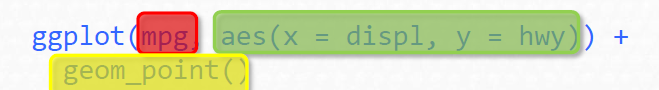
\includegraphics{images/basic_ggplot.png}
\end{itemize}
\end{frame}

\begin{frame}[fragile]{Basic Structure. Points}
\phantomsection\label{basic-structure.-points}
\begin{Shaded}
\begin{Highlighting}[]
\FunctionTok{library}\NormalTok{(ggplot2)}
\FunctionTok{ggplot}\NormalTok{(osteo, }\FunctionTok{aes}\NormalTok{(}\AttributeTok{x =}\NormalTok{ edad , }\AttributeTok{y =}\NormalTok{ bua )) }\SpecialCharTok{+} 
  \FunctionTok{geom\_point}\NormalTok{()}
\end{Highlighting}
\end{Shaded}

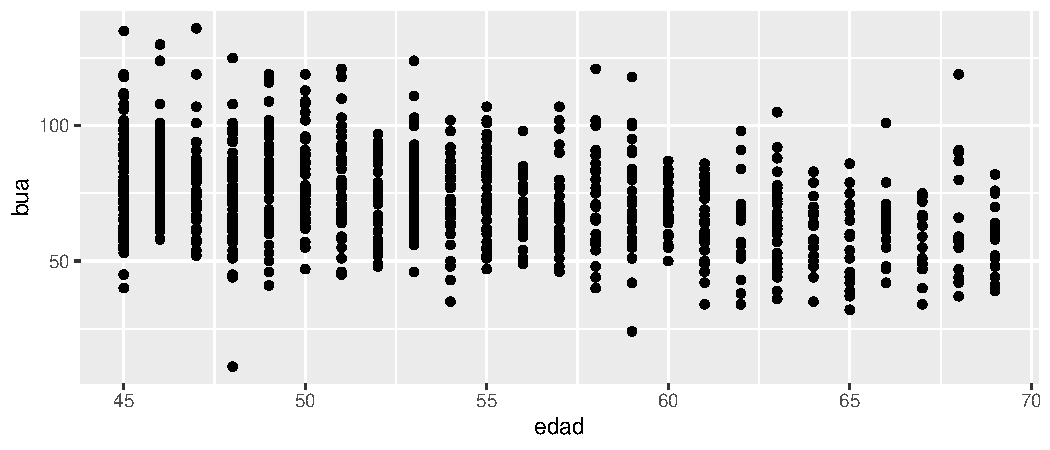
\includegraphics{StatisticsWithR-3-Exploratory_Analysis_II_And_Graphics_files/figure-beamer/unnamed-chunk-4-1.pdf}
\end{frame}

\begin{frame}[fragile]{Basic Structure. Points + color}
\phantomsection\label{basic-structure.-points-color}
\begin{Shaded}
\begin{Highlighting}[]
\FunctionTok{ggplot}\NormalTok{(osteo, }\FunctionTok{aes}\NormalTok{(}\AttributeTok{x =}\NormalTok{ edad , }\AttributeTok{y =}\NormalTok{ bua   , }\AttributeTok{color =}\NormalTok{ menop)) }\SpecialCharTok{+} 
  \FunctionTok{geom\_point}\NormalTok{()}
\end{Highlighting}
\end{Shaded}

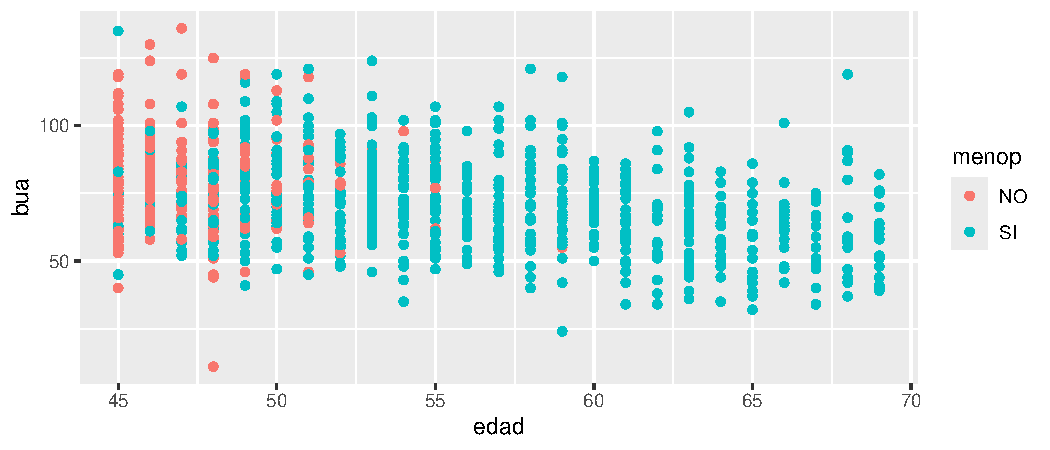
\includegraphics{StatisticsWithR-3-Exploratory_Analysis_II_And_Graphics_files/figure-beamer/unnamed-chunk-5-1.pdf}
\end{frame}

\begin{frame}[fragile]{Basic Structure. Points + color + shape}
\phantomsection\label{basic-structure.-points-color-shape}
\begin{Shaded}
\begin{Highlighting}[]
\FunctionTok{ggplot}\NormalTok{(osteo, }\FunctionTok{aes}\NormalTok{(}\AttributeTok{x =}\NormalTok{ edad , }\AttributeTok{y =}\NormalTok{ bua   , }\AttributeTok{color =}\NormalTok{ menop, }\AttributeTok{shape =}\NormalTok{ clasific )) }\SpecialCharTok{+} 
  \FunctionTok{geom\_point}\NormalTok{()}
\end{Highlighting}
\end{Shaded}

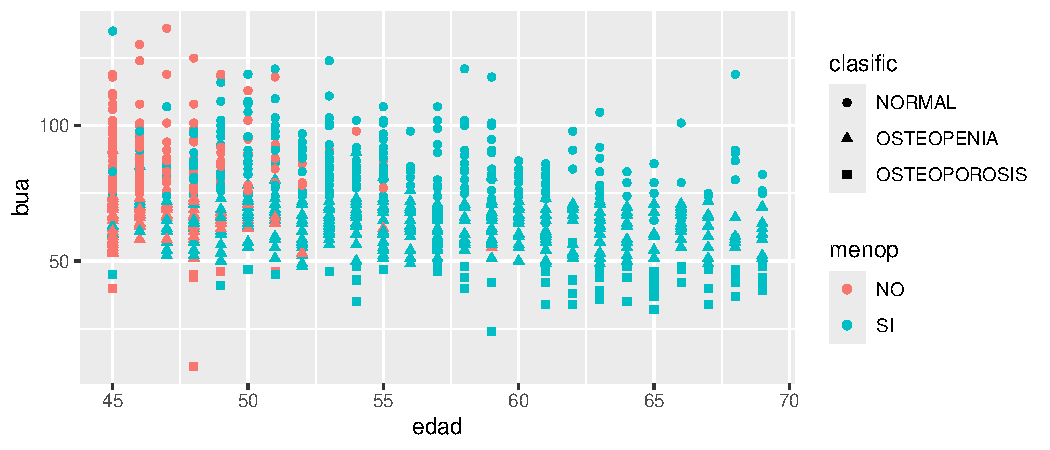
\includegraphics{StatisticsWithR-3-Exploratory_Analysis_II_And_Graphics_files/figure-beamer/unnamed-chunk-6-1.pdf}
\end{frame}

\section{From Univariate to Bivariate
Analysis}\label{from-univariate-to-bivariate-analysis}

\begin{frame}{From Univariate to Bivariate Analysis}
\begin{itemize}
\item
  Elegant graphics for data analysis
\item
  \textbf{From univariate to bivariate analysis}
\item
  Bivariate analysis

  \begin{itemize}
  \item
    Qualitative vs Qualitative
  \item
    Qualitative vs Quantitative
  \item
    Quantitative vs Quantitative
  \end{itemize}
\item
  Correlation

  \begin{itemize}
  \item
    Definition
  \item
    Types of correlation (Pearson, Spearman)
  \end{itemize}
\item
  Extra
\end{itemize}
\end{frame}

\section{From Univariate to Bivariate
Analysis}\label{from-univariate-to-bivariate-analysis-1}

\begin{frame}{From Univariate to Bivariate Analysis}
\begin{itemize}
\tightlist
\item
  Univariate: analysis of one variable
\item
  Bivariate: check for relationships between two variables
\end{itemize}
\end{frame}

\begin{frame}{Questions to consider}
\phantomsection\label{questions-to-consider}
If there are more than one variable in the dataset it could be
interesting to guess if:

\begin{itemize}
\tightlist
\item
  Does a relation exist?
\item
  How important is it?
\item
  What is the direction?
\end{itemize}
\end{frame}

\section{Bivariate Analysis}\label{bivariate-analysis}

\begin{frame}{Bivariate Analysis}
\begin{itemize}
\item
  Elegant graphics for data analysis
\item
  From univariate to bivariate analysis
\item
  \textbf{Bivariate analysis}

  \begin{itemize}
  \item
    \textbf{Qualitative vs Qualitative}
  \item
    \textbf{Qualitative vs Quantitative}
  \item
    \textbf{Quantitative vs Quantitative}
  \end{itemize}
\item
  Correlation

  \begin{itemize}
  \item
    Definition
  \item
    Types of correlation (Pearson, Spearman)
  \end{itemize}
\item
  Extra
\end{itemize}
\end{frame}

\section{Bivariate Analysis}\label{bivariate-analysis-1}

\begin{frame}{Types}
\phantomsection\label{types}
Some plots to study the relationship between two variables\ldots{}

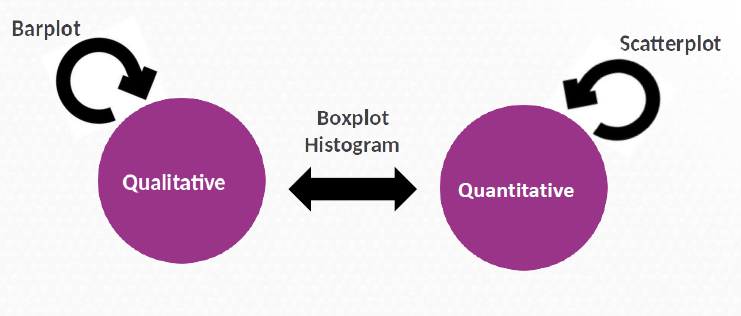
\includegraphics{images/types.png}
\end{frame}

\begin{frame}{Definition}
\phantomsection\label{definition}
\begin{itemize}
\tightlist
\item
  Bivariate analysis explores the relationship between two variables.
\item
  The approach depends on whether the variables are numerical or
  categorical.
\end{itemize}
\end{frame}

\begin{frame}[fragile]{Qualitative vs Qualitative}
\phantomsection\label{qualitative-vs-qualitative}
\begin{itemize}
\tightlist
\item
  Use contingency tables
\item
  Chi-squared test for independence
\end{itemize}

\begin{block}{Example data}
\phantomsection\label{example-data}
\begin{Shaded}
\begin{Highlighting}[]
\FunctionTok{library}\NormalTok{(rio)}
\FunctionTok{library}\NormalTok{(gmodels)}

\FunctionTok{CrossTable}\NormalTok{(osteo}\SpecialCharTok{$}\NormalTok{grupedad, osteo}\SpecialCharTok{$}\NormalTok{clasific, }\AttributeTok{prop.c =} \ConstantTok{FALSE}\NormalTok{, }\AttributeTok{prop.r =} \ConstantTok{FALSE}\NormalTok{, }\AttributeTok{prop.chisq =} \ConstantTok{FALSE}\NormalTok{)}
\end{Highlighting}
\end{Shaded}

\begin{verbatim}
## 
##  
##    Cell Contents
## |-------------------------|
## |                       N |
## |         N / Table Total |
## |-------------------------|
## 
##  
## Total Observations in Table:  1000 
## 
##  
##                | osteo$clasific 
## osteo$grupedad |       NORMAL |   OSTEOPENIA | OSTEOPOROSIS |    Row Total | 
## ---------------|--------------|--------------|--------------|--------------|
##        45 - 49 |          233 |          138 |            7 |          378 | 
##                |        0.233 |        0.138 |        0.007 |              | 
## ---------------|--------------|--------------|--------------|--------------|
##        50 - 54 |          113 |          113 |            7 |          233 | 
##                |        0.113 |        0.113 |        0.007 |              | 
## ---------------|--------------|--------------|--------------|--------------|
##        55 - 59 |           67 |          100 |            9 |          176 | 
##                |        0.067 |        0.100 |        0.009 |              | 
## ---------------|--------------|--------------|--------------|--------------|
##        60 - 64 |           38 |           74 |           17 |          129 | 
##                |        0.038 |        0.074 |        0.017 |              | 
## ---------------|--------------|--------------|--------------|--------------|
##        65 - 69 |           18 |           42 |           24 |           84 | 
##                |        0.018 |        0.042 |        0.024 |              | 
## ---------------|--------------|--------------|--------------|--------------|
##   Column Total |          469 |          467 |           64 |         1000 | 
## ---------------|--------------|--------------|--------------|--------------|
## 
## 
\end{verbatim}
\end{block}
\end{frame}

\begin{frame}[fragile]{Barplots}
\phantomsection\label{barplots}
\begin{itemize}
\tightlist
\item
  We can use bar plots to explore the relationship.
\item
  Example: \textbf{grupedad vs clasific}
\end{itemize}

\begin{Shaded}
\begin{Highlighting}[]
\FunctionTok{ggplot}\NormalTok{(osteo, }\FunctionTok{aes}\NormalTok{(}\AttributeTok{x =}\NormalTok{ grupedad, }\AttributeTok{fill =}\NormalTok{ clasific)) }\SpecialCharTok{+} 
  \FunctionTok{geom\_bar}\NormalTok{()}
\end{Highlighting}
\end{Shaded}

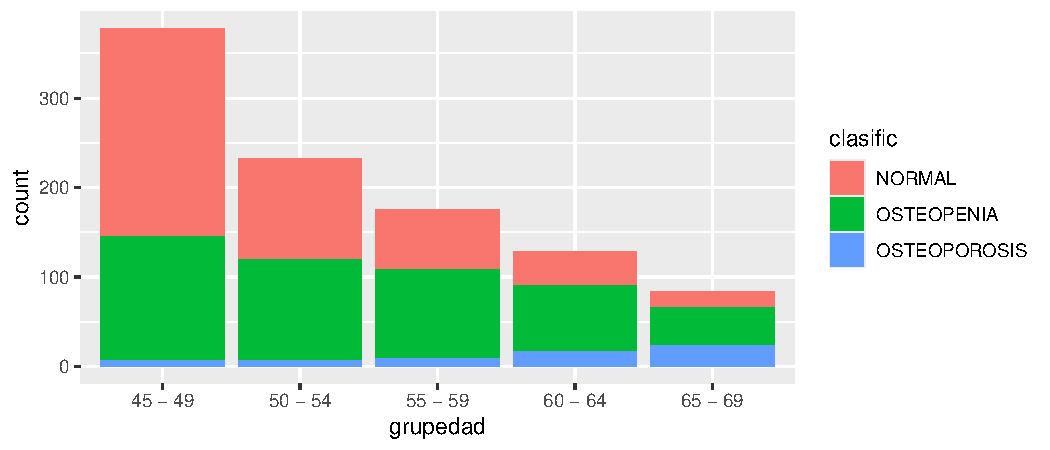
\includegraphics{StatisticsWithR-3-Exploratory_Analysis_II_And_Graphics_files/figure-beamer/unnamed-chunk-8-1.pdf}

\begin{Shaded}
\begin{Highlighting}[]
\FunctionTok{ggplot}\NormalTok{(osteo, }\FunctionTok{aes}\NormalTok{(}\AttributeTok{x =}\NormalTok{ grupedad, }\AttributeTok{fill =}\NormalTok{ clasific)) }\SpecialCharTok{+} 
  \FunctionTok{geom\_bar}\NormalTok{(}\AttributeTok{position =} \StringTok{"dodge"}\NormalTok{)}
\end{Highlighting}
\end{Shaded}

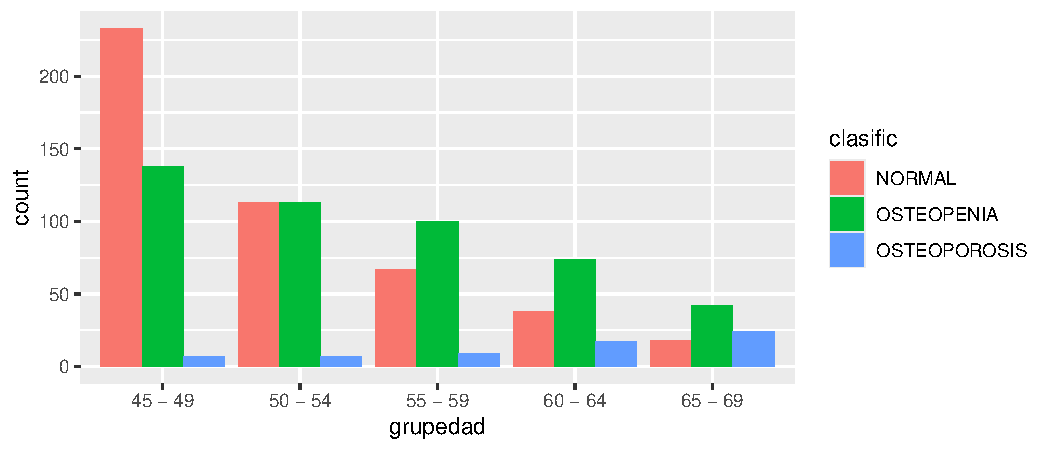
\includegraphics{StatisticsWithR-3-Exploratory_Analysis_II_And_Graphics_files/figure-beamer/unnamed-chunk-9-1.pdf}
\end{frame}

\begin{frame}[fragile]{Customizing}
\phantomsection\label{customizing}
\begin{Shaded}
\begin{Highlighting}[]
\NormalTok{p }\OtherTok{\textless{}{-}} \FunctionTok{ggplot}\NormalTok{(osteo, }\FunctionTok{aes}\NormalTok{(}\AttributeTok{x =}\NormalTok{ grupedad, }\AttributeTok{fill =}\NormalTok{ clasific)) }\SpecialCharTok{+}
  \FunctionTok{geom\_bar}\NormalTok{(}\AttributeTok{position =} \StringTok{"dodge"}\NormalTok{) }\SpecialCharTok{+}
  \FunctionTok{scale\_fill\_manual}\NormalTok{(}\AttributeTok{values=}\FunctionTok{c}\NormalTok{(}\StringTok{"\#8618b1"}\NormalTok{, }\StringTok{"blanchedalmond"}\NormalTok{, }\StringTok{"red"}\NormalTok{)) }\SpecialCharTok{+}
  \FunctionTok{theme}\NormalTok{(}\AttributeTok{legend.position=}\StringTok{"bottom"}\NormalTok{) }\SpecialCharTok{+}
  \FunctionTok{labs}\NormalTok{(}\AttributeTok{x =} \StringTok{"Age group"}\NormalTok{, }\AttributeTok{y =} \StringTok{"Women"}\NormalTok{, }\AttributeTok{title =} \StringTok{"Osteo disease classified by age group"}\NormalTok{)}
\NormalTok{p}
\end{Highlighting}
\end{Shaded}

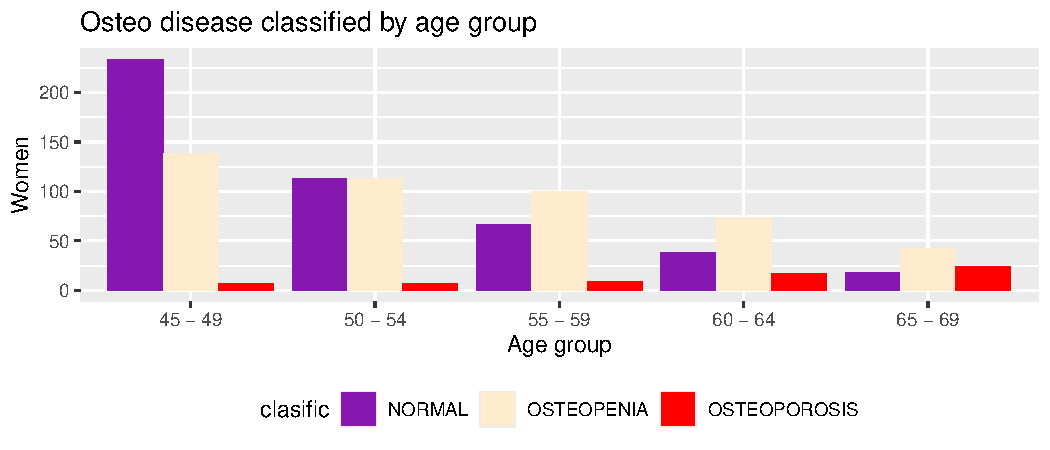
\includegraphics{StatisticsWithR-3-Exploratory_Analysis_II_And_Graphics_files/figure-beamer/unnamed-chunk-10-1.pdf}
\end{frame}

\begin{frame}[fragile]{Qualitative vs Quantitative}
\phantomsection\label{qualitative-vs-quantitative}
\begin{itemize}
\tightlist
\item
  One qualitative and one quantitative variable
\item
  Use table of means or boxplots
\end{itemize}

\begin{Shaded}
\begin{Highlighting}[]
\FunctionTok{library}\NormalTok{(dplyr)}
\end{Highlighting}
\end{Shaded}

\begin{verbatim}
## 
## Adjuntando el paquete: 'dplyr'
\end{verbatim}

\begin{verbatim}
## The following objects are masked from 'package:stats':
## 
##     filter, lag
\end{verbatim}

\begin{verbatim}
## The following objects are masked from 'package:base':
## 
##     intersect, setdiff, setequal, union
\end{verbatim}

\begin{Shaded}
\begin{Highlighting}[]
\NormalTok{osteo }\SpecialCharTok{\%\textgreater{}\%}
  \FunctionTok{group\_by}\NormalTok{(grupedad) }\SpecialCharTok{\%\textgreater{}\%}
  \FunctionTok{summarize}\NormalTok{(}\AttributeTok{mean\_bua =} \FunctionTok{mean}\NormalTok{(bua, }\AttributeTok{na.rm =} \ConstantTok{TRUE}\NormalTok{))}
\end{Highlighting}
\end{Shaded}

\begin{verbatim}
## # A tibble: 5 x 2
##   grupedad mean_bua
##   <chr>       <dbl>
## 1 45 - 49      78.8
## 2 50 - 54      75.1
## 3 55 - 59      71.4
## 4 60 - 64      64.9
## 5 65 - 69      60.7
\end{verbatim}
\end{frame}

\begin{frame}[fragile]{Boxplots}
\phantomsection\label{boxplots}
\begin{Shaded}
\begin{Highlighting}[]
\NormalTok{bp }\OtherTok{\textless{}{-}} \FunctionTok{ggplot}\NormalTok{(osteo, }\FunctionTok{aes}\NormalTok{(}\AttributeTok{x =}\NormalTok{ grupedad, }\AttributeTok{y =}\NormalTok{ bua)) }\SpecialCharTok{+} 
  \FunctionTok{geom\_boxplot}\NormalTok{(}\AttributeTok{fill =} \StringTok{\textquotesingle{}\#A4A4A4\textquotesingle{}}\NormalTok{, }\AttributeTok{color =} \StringTok{"purple"}\NormalTok{)}
\NormalTok{bp}
\end{Highlighting}
\end{Shaded}

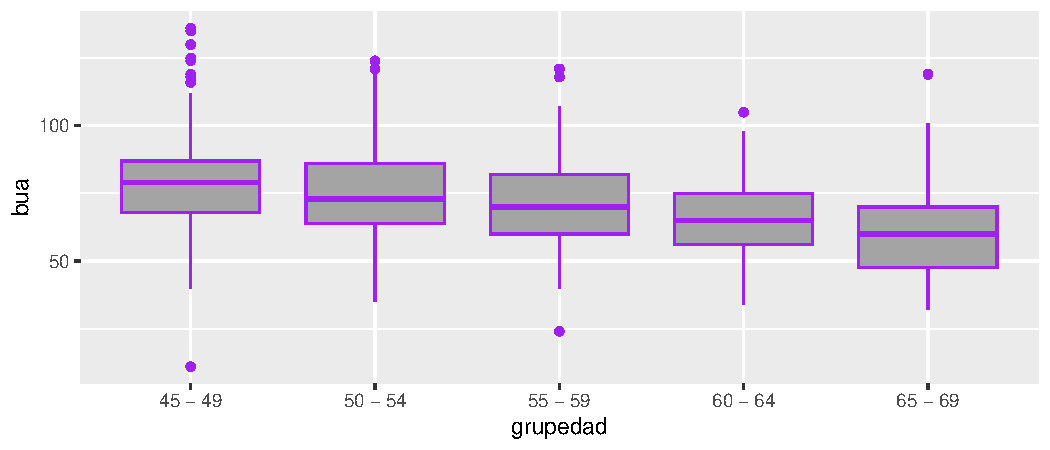
\includegraphics{StatisticsWithR-3-Exploratory_Analysis_II_And_Graphics_files/figure-beamer/unnamed-chunk-12-1.pdf}
\end{frame}

\begin{frame}[fragile]{Customizing}
\phantomsection\label{customizing-1}
\begin{Shaded}
\begin{Highlighting}[]
\NormalTok{bp }\SpecialCharTok{+} \FunctionTok{geom\_jitter}\NormalTok{(}\AttributeTok{shape =} \DecValTok{16}\NormalTok{, }\AttributeTok{position =} \FunctionTok{position\_jitter}\NormalTok{(}\FloatTok{0.2}\NormalTok{)) }\SpecialCharTok{+}
  \FunctionTok{labs}\NormalTok{(}\AttributeTok{x =} \StringTok{"Age Group"}\NormalTok{, }\AttributeTok{y =} \StringTok{"Women"}\NormalTok{, }\AttributeTok{title =} \StringTok{"Osteo disease classified by age group"}\NormalTok{)}
\end{Highlighting}
\end{Shaded}

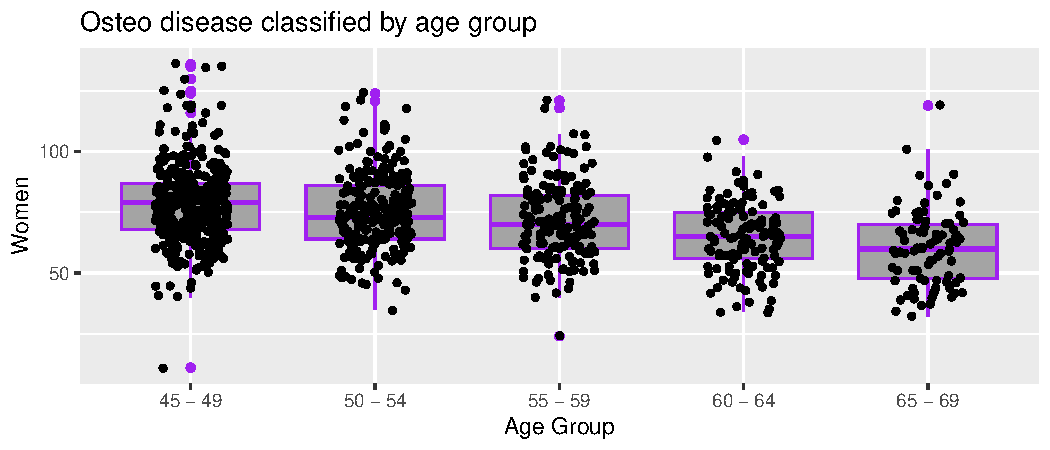
\includegraphics{StatisticsWithR-3-Exploratory_Analysis_II_And_Graphics_files/figure-beamer/unnamed-chunk-13-1.pdf}
\end{frame}

\begin{frame}[fragile]{Quantitative vs Quantitative}
\phantomsection\label{quantitative-vs-quantitative}
\begin{itemize}
\tightlist
\item
  Scatter plots are useful to show correlation or pattern.
\item
  Example: \textbf{edad vs bua}
\end{itemize}

\begin{block}{Example data}
\phantomsection\label{example-data-1}
\begin{Shaded}
\begin{Highlighting}[]
\FunctionTok{head}\NormalTok{(osteo[, }\FunctionTok{c}\NormalTok{(}\StringTok{"peso"}\NormalTok{, }\StringTok{"imc"}\NormalTok{)], }\AttributeTok{n =} \DecValTok{10}\NormalTok{)}
\end{Highlighting}
\end{Shaded}

\begin{verbatim}
##    peso   imc
## 1  70.0 24.80
## 2  53.0 22.94
## 3  64.0 25.64
## 4  78.0 30.09
## 5  56.0 22.72
## 6  63.5 21.97
## 7  86.0 33.18
## 8  61.5 22.87
## 9  60.5 24.23
## 10 64.0 28.83
\end{verbatim}
\end{block}
\end{frame}

\begin{frame}[fragile]{Scatterplot}
\phantomsection\label{scatterplot}
\begin{Shaded}
\begin{Highlighting}[]
\FunctionTok{ggplot}\NormalTok{(osteo, }\FunctionTok{aes}\NormalTok{(}\AttributeTok{x =}\NormalTok{ peso, }\AttributeTok{y =}\NormalTok{ imc)) }\SpecialCharTok{+} 
  \FunctionTok{geom\_point}\NormalTok{()}
\end{Highlighting}
\end{Shaded}

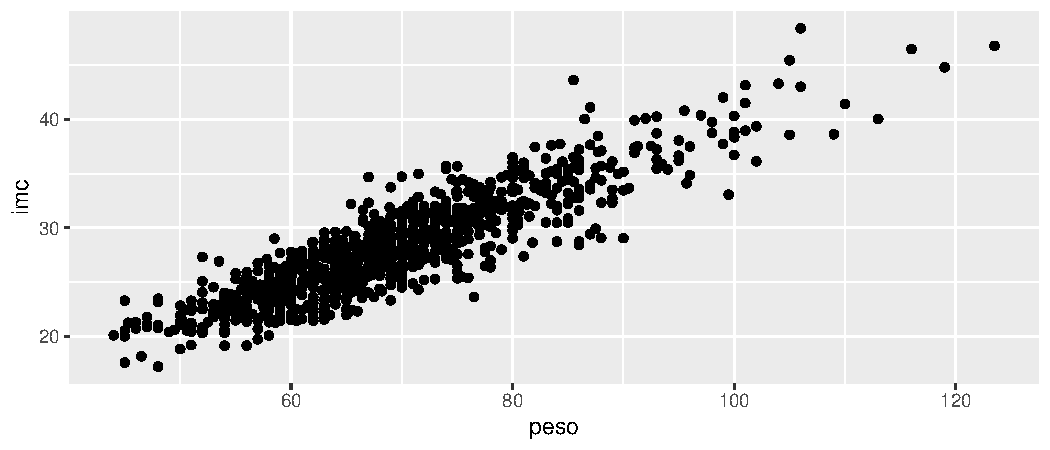
\includegraphics{StatisticsWithR-3-Exploratory_Analysis_II_And_Graphics_files/figure-beamer/unnamed-chunk-15-1.pdf}
\end{frame}

\begin{frame}[fragile]{Customizing}
\phantomsection\label{customizing-2}
\begin{Shaded}
\begin{Highlighting}[]
\FunctionTok{ggplot}\NormalTok{(osteo, }\FunctionTok{aes}\NormalTok{(}\AttributeTok{x =}\NormalTok{ peso, }\AttributeTok{y =}\NormalTok{ imc)) }\SpecialCharTok{+}
  \FunctionTok{geom\_point}\NormalTok{(}\AttributeTok{size =} \DecValTok{1}\NormalTok{, }\AttributeTok{shape =} \DecValTok{1}\NormalTok{)}
\end{Highlighting}
\end{Shaded}

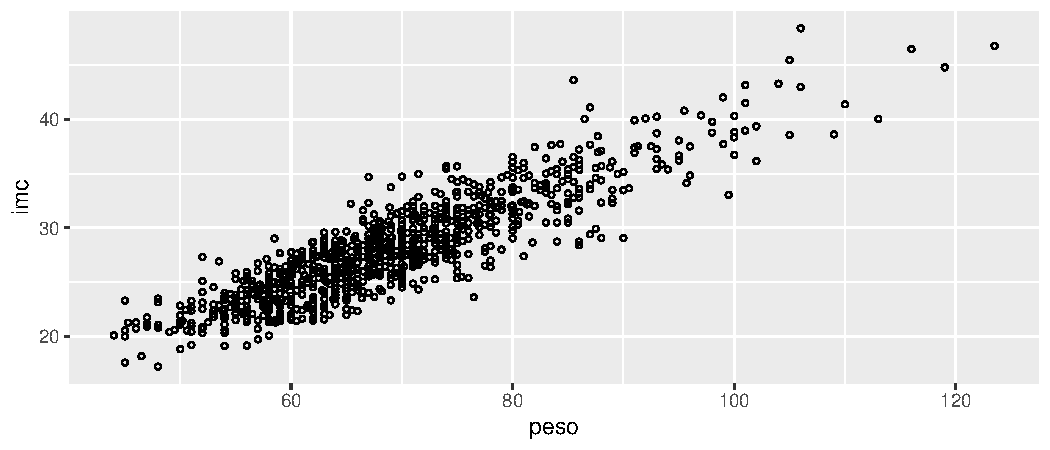
\includegraphics{StatisticsWithR-3-Exploratory_Analysis_II_And_Graphics_files/figure-beamer/unnamed-chunk-16-1.pdf}
\end{frame}

\begin{frame}[fragile]{Add information}
\phantomsection\label{add-information}
\begin{Shaded}
\begin{Highlighting}[]
\FunctionTok{ggplot}\NormalTok{(osteo, }\FunctionTok{aes}\NormalTok{(}\AttributeTok{x =}\NormalTok{ peso, }\AttributeTok{y =}\NormalTok{ imc, }\AttributeTok{color =}\NormalTok{ clasific, }\AttributeTok{shape =}\NormalTok{ clasific)) }\SpecialCharTok{+}
  \FunctionTok{geom\_point}\NormalTok{()}
\end{Highlighting}
\end{Shaded}

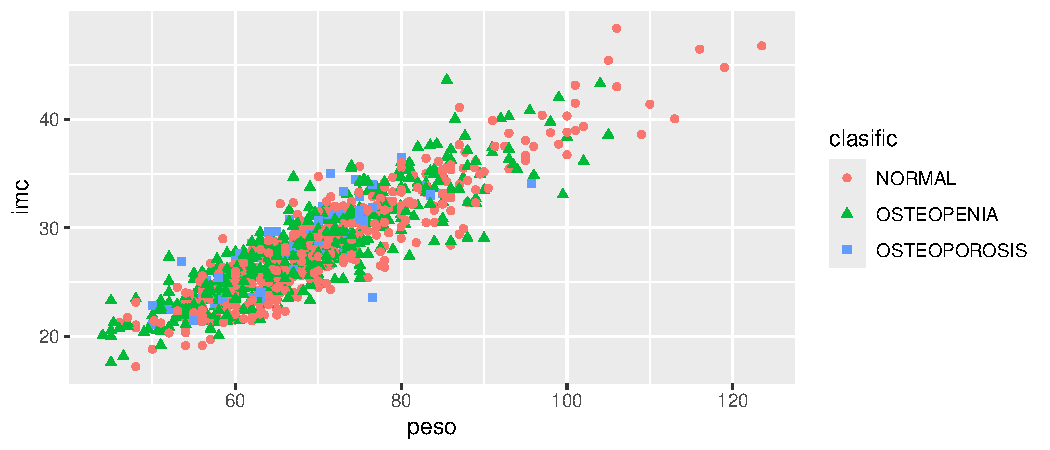
\includegraphics{StatisticsWithR-3-Exploratory_Analysis_II_And_Graphics_files/figure-beamer/unnamed-chunk-17-1.pdf}
\end{frame}

\begin{frame}[fragile]{Other relation}
\phantomsection\label{other-relation}
But not always the correlation is good!

\begin{Shaded}
\begin{Highlighting}[]
\FunctionTok{ggplot}\NormalTok{(osteo, }\FunctionTok{aes}\NormalTok{(}\AttributeTok{x =}\NormalTok{ edad, }\AttributeTok{y =}\NormalTok{ imc)) }\SpecialCharTok{+}
  \FunctionTok{geom\_point}\NormalTok{()}
\end{Highlighting}
\end{Shaded}

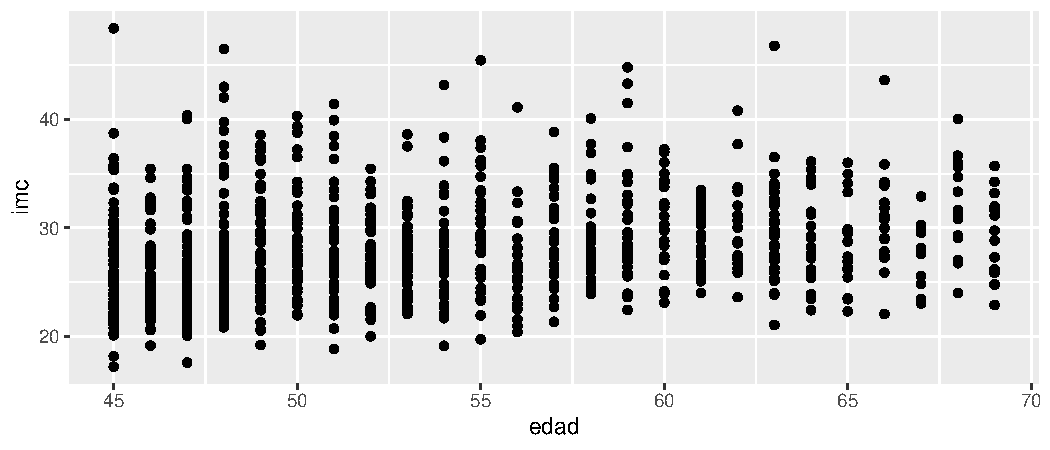
\includegraphics{StatisticsWithR-3-Exploratory_Analysis_II_And_Graphics_files/figure-beamer/unnamed-chunk-18-1.pdf}
\end{frame}

\begin{frame}[fragile]{Multiple plots}
\phantomsection\label{multiple-plots}
\begin{Shaded}
\begin{Highlighting}[]
\FunctionTok{library}\NormalTok{(GGally)}
\end{Highlighting}
\end{Shaded}

\begin{verbatim}
## Registered S3 method overwritten by 'GGally':
##   method from   
##   +.gg   ggplot2
\end{verbatim}

\begin{Shaded}
\begin{Highlighting}[]
\FunctionTok{ggpairs}\NormalTok{(osteo, }\AttributeTok{columns =} \FunctionTok{c}\NormalTok{(}\StringTok{"edad"}\NormalTok{, }\StringTok{"peso"}\NormalTok{, }\StringTok{"talla"}\NormalTok{, }\StringTok{"imc"}\NormalTok{, }\StringTok{"bua"}\NormalTok{, }\StringTok{"menarqui"}\NormalTok{), }
\NormalTok{        ggplot2}\SpecialCharTok{::}\FunctionTok{aes}\NormalTok{(}\AttributeTok{colour =}\NormalTok{ clasific))}
\end{Highlighting}
\end{Shaded}

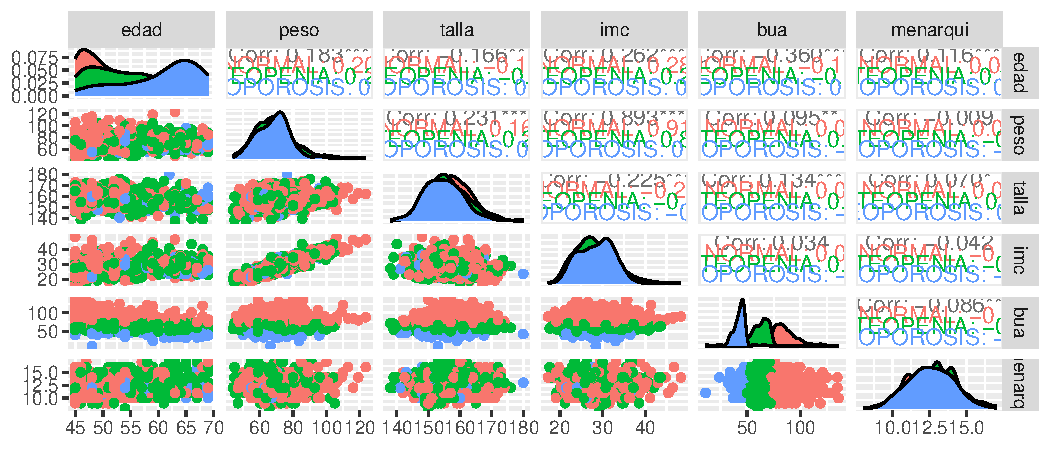
\includegraphics{StatisticsWithR-3-Exploratory_Analysis_II_And_Graphics_files/figure-beamer/unnamed-chunk-19-1.pdf}
\end{frame}

\section{Exercise I}\label{exercise-i}

\begin{frame}[fragile]{Exercise I}
Load the \texttt{diabetes} dataset

\begin{Shaded}
\begin{Highlighting}[]
\FunctionTok{p\_load}\NormalTok{(janitor)}
\NormalTok{  diab }\OtherTok{\textless{}{-}} \FunctionTok{import}\NormalTok{(}\StringTok{"datasets/diabetes\_mod.xls"}\NormalTok{)}
\NormalTok{diab}\OtherTok{\textless{}{-}} \FunctionTok{clean\_names}\NormalTok{(diab)}
\end{Highlighting}
\end{Shaded}

Study relation between \texttt{mort} and \texttt{tabac}

\begin{itemize}
\item
  \textbf{Build a contingency table between \texttt{mort} and
  \texttt{tabac}.}
\item
  \textbf{Visualize the relationship between \texttt{mort} and
  \texttt{tabac}.}
\end{itemize}

Study relation between \texttt{mort} and \texttt{bmi}

\begin{itemize}
\item
  \textbf{Calculate Mean, median, and standard deviation of bmi by
  categories of mort.}
\item
  \textbf{Visualze the relationship between \texttt{bmi} by
  \texttt{mort} status}
\end{itemize}

Study relation between \texttt{bmi} and \texttt{edad}

\begin{itemize}
\tightlist
\item
  \textbf{Visualze the relationship between age and BMI.}
\end{itemize}

Is there a relationship between the variables?
\end{frame}

\section{Correlation}\label{correlation}

\begin{frame}{Correlation}
\begin{itemize}
\item
  Elegant graphics for data analysis
\item
  From univariate to bivariate analysis
\item
  Bivariate analysis

  \begin{itemize}
  \item
    Qualitative vs Qualitative
  \item
    Qualitative vs Quantitative
  \item
    Quantitative vs Quantitative
  \end{itemize}
\item
  \textbf{Correlation}

  \begin{itemize}
  \item
    \textbf{Definition}
  \item
    \textbf{Types of correlation (Pearson, Spearman)}
  \end{itemize}
\item
  Extra
\end{itemize}
\end{frame}

\section{Correlation}\label{correlation-1}

\begin{frame}{Main characteristics}
\phantomsection\label{main-characteristics}
Correlation analysis allows

\begin{itemize}
\item
  To study the way of relation between the two variables
\item
  To quantify the intensity of relation
\end{itemize}

Correlation is not causation one thing does not causes the other

In the correlation analysis, the two variables have the same weight

The correlation coefficient measures the strength of a linear relation
\end{frame}

\begin{frame}{Concepts}
\phantomsection\label{concepts}
\begin{itemize}
\tightlist
\item
  Correlation quantifies strength and direction of relationship
\item
  r from -1 to 1

  \begin{itemize}
  \tightlist
  \item
    r \textgreater{} 0: direct
  \item
    r \textless{} 0: inverse
  \item
    r = 0: no relation
  \end{itemize}
\end{itemize}
\end{frame}

\begin{frame}{Types correlation. Pearson}
\phantomsection\label{types-correlation.-pearson}
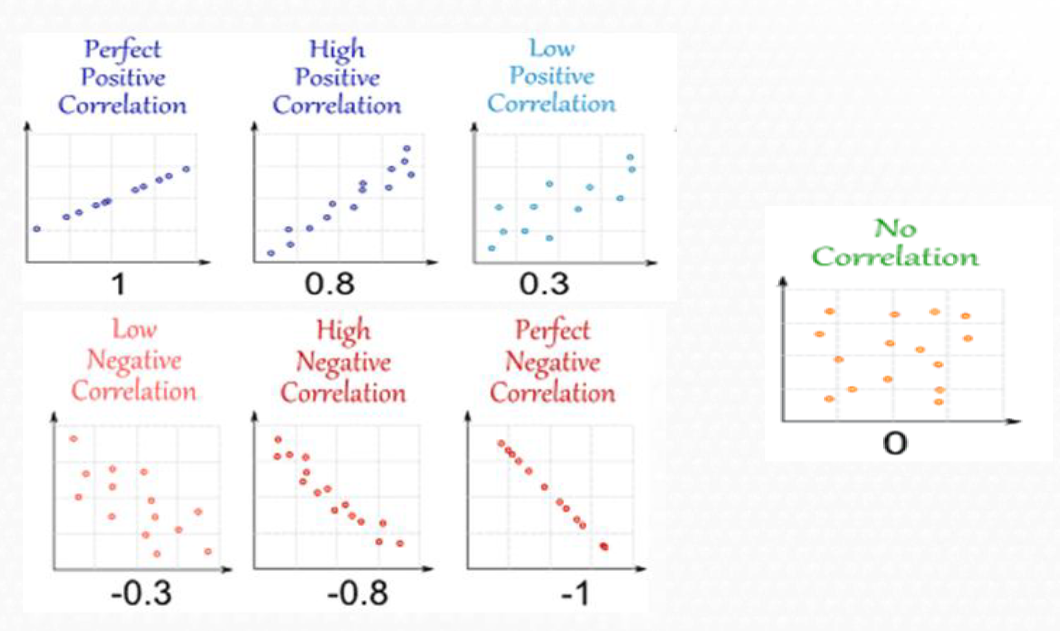
\includegraphics{images/types_correlation.png}
\end{frame}

\begin{frame}[fragile]{Pearson}
\phantomsection\label{pearson}
\begin{Shaded}
\begin{Highlighting}[]
\FunctionTok{cor}\NormalTok{(osteo}\SpecialCharTok{$}\NormalTok{bua, osteo}\SpecialCharTok{$}\NormalTok{edad, }\AttributeTok{method =} \StringTok{"pearson"}\NormalTok{)}
\end{Highlighting}
\end{Shaded}

\begin{verbatim}
## [1] -0.3601883
\end{verbatim}

Don't forget to look the graphic!!

\begin{Shaded}
\begin{Highlighting}[]
\FunctionTok{ggplot}\NormalTok{(osteo, }\FunctionTok{aes}\NormalTok{(}\AttributeTok{x =}\NormalTok{ edad, }\AttributeTok{y =}\NormalTok{ bua)) }\SpecialCharTok{+} 
  \FunctionTok{geom\_point}\NormalTok{()}
\end{Highlighting}
\end{Shaded}

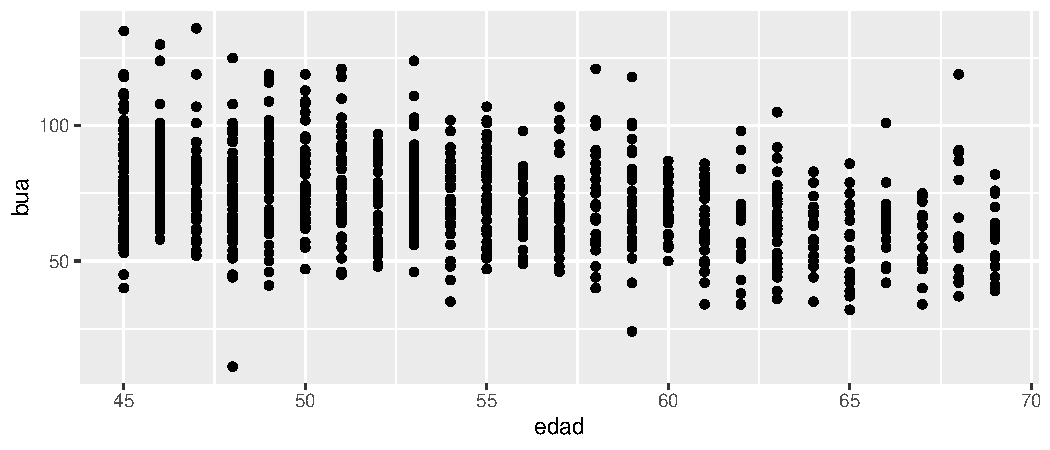
\includegraphics{StatisticsWithR-3-Exploratory_Analysis_II_And_Graphics_files/figure-beamer/unnamed-chunk-22-1.pdf}
\end{frame}

\begin{frame}{Spearman}
\phantomsection\label{spearman}
\begin{itemize}
\tightlist
\item
  Pearson correlation coefficient is severely affected by outliers and
  if the relation is not linear
\end{itemize}

--\textgreater{} Better to use Spearman correlation coefficient (use the
ranks between the numbers instead the values) to calculate the
correlation coefficient

\begin{itemize}
\tightlist
\item
  Evaluates the monotonic relationship between the variables (not the
  linear relationship as Pearson does).
\end{itemize}

--\textgreater The variables tend to change together but not necessarily
at a constant rate

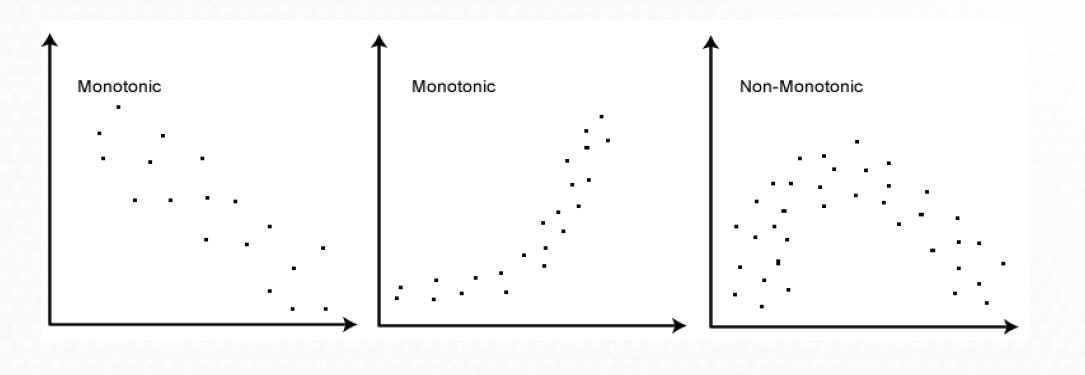
\includegraphics{images/spearman.png}
\end{frame}

\begin{frame}{Types of correlation}
\phantomsection\label{types-of-correlation}
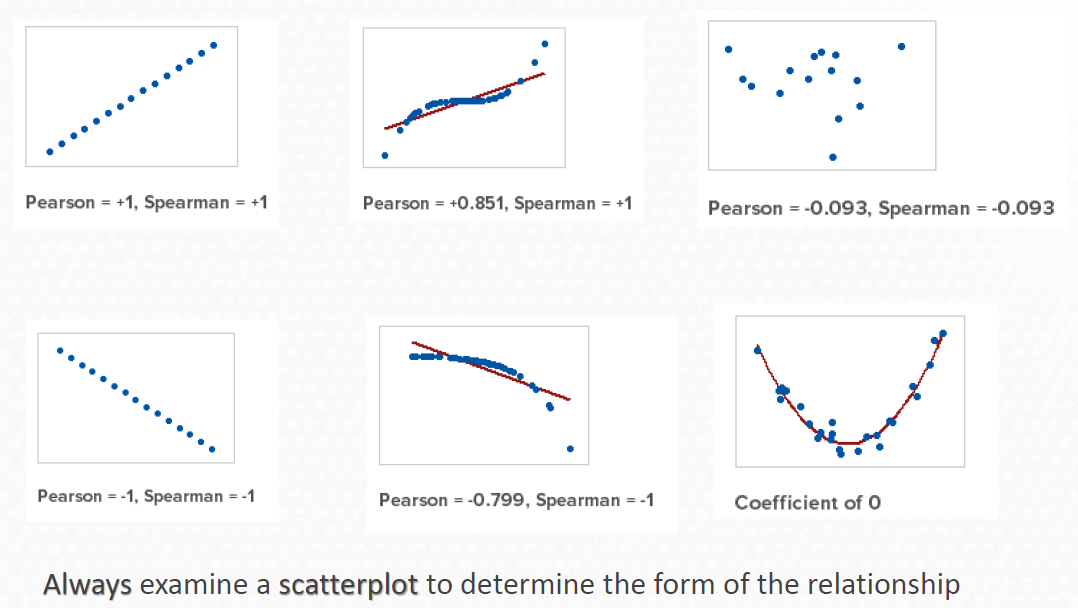
\includegraphics{images/comparison_correlation.png}
\end{frame}

\begin{frame}[fragile]{Example}
\phantomsection\label{example}
\begin{Shaded}
\begin{Highlighting}[]
\FunctionTok{cor}\NormalTok{(osteo}\SpecialCharTok{$}\NormalTok{bua, osteo}\SpecialCharTok{$}\NormalTok{edad, }\AttributeTok{method =} \StringTok{"spearman"}\NormalTok{)}
\end{Highlighting}
\end{Shaded}

\begin{verbatim}
## [1] -0.3540295
\end{verbatim}
\end{frame}

\begin{frame}[fragile]{Correlation Matrix}
\phantomsection\label{correlation-matrix}
\begin{Shaded}
\begin{Highlighting}[]
\FunctionTok{cor}\NormalTok{(osteo[, }\FunctionTok{c}\NormalTok{(}\StringTok{"edad"}\NormalTok{, }\StringTok{"peso"}\NormalTok{, }\StringTok{"talla"}\NormalTok{, }\StringTok{"imc"}\NormalTok{, }\StringTok{"bua"}\NormalTok{, }\StringTok{"menarqui"}\NormalTok{)], }\AttributeTok{use =} \StringTok{"complete.obs"}\NormalTok{)}
\end{Highlighting}
\end{Shaded}

\begin{verbatim}
##                edad         peso       talla         imc         bua
## edad      1.0000000  0.182629245 -0.16635268  0.26173285 -0.36018834
## peso      0.1826292  1.000000000  0.23110585  0.89278635  0.09467837
## talla    -0.1663527  0.231105848  1.00000000 -0.22546438  0.13350207
## imc       0.2617329  0.892786346 -0.22546438  1.00000000  0.03415938
## bua      -0.3601883  0.094678365  0.13350207  0.03415938  1.00000000
## menarqui  0.1159013 -0.008526465  0.07000284 -0.04160766 -0.08593554
##              menarqui
## edad      0.115901253
## peso     -0.008526465
## talla     0.070002843
## imc      -0.041607661
## bua      -0.085935539
## menarqui  1.000000000
\end{verbatim}
\end{frame}

\section{Summary}\label{summary}

\begin{frame}[fragile]{Summary}
\begin{itemize}
\tightlist
\item
  Use \texttt{geom\_bar} for categorical-categorical
\item
  Use \texttt{geom\_boxplot} for categorical-numerical
\item
  Use \texttt{geom\_point} for numerical-numerical
\item
  Always include clear labels and titles
\end{itemize}
\end{frame}

\section{Exercises II}\label{exercises-ii}

\begin{frame}[fragile]{Exercises II}
\begin{itemize}
\tightlist
\item
  \textbf{Calculate Pearson and Spearman correlations between
  \texttt{edat} and \texttt{bmi}.}
\end{itemize}

\textbf{Scatter plot of \texttt{edat} vs \texttt{bmi} colored by CHD
status.}

\begin{itemize}
\item
  \textbf{Calculate the correlation between all pairs of numerical
  variables.}
\item
  \textbf{Use the GGally package to visualize all pairwise relationships
  between variables using the ggpairs() function.}
\end{itemize}
\end{frame}

\section{Extra}\label{extra}

\begin{frame}{Extra}
\begin{itemize}
\item
  Elegant graphics for data analysis
\item
  From univariate to bivariate analysis
\item
  Bivariate analysis

  \begin{itemize}
  \item
    Qualitative vs Qualitative
  \item
    Qualitative vs Quantitative
  \item
    Quantitative vs Quantitative
  \end{itemize}
\item
  Correlation

  \begin{itemize}
  \item
    Definition
  \item
    Types of correlation (Pearson, Spearman)
  \end{itemize}
\item
  \textbf{Extra}
\end{itemize}
\end{frame}

\section{Extra}\label{extra-1}

\section{Interactive and Impressive
Plots}\label{interactive-and-impressive-plots}

\begin{frame}[fragile]{Interactive Scatter Plot with Tooltips}
\phantomsection\label{interactive-scatter-plot-with-tooltips}
\begin{Shaded}
\begin{Highlighting}[]
\FunctionTok{p\_load}\NormalTok{(plotly)}

\NormalTok{p1 }\OtherTok{\textless{}{-}} \FunctionTok{ggplot}\NormalTok{(diab, }\FunctionTok{aes}\NormalTok{(}\AttributeTok{x =}\NormalTok{ edat, }\AttributeTok{y =}\NormalTok{ bmi, }\AttributeTok{color =}\NormalTok{ tabac, }\AttributeTok{label =}\NormalTok{ chd)) }\SpecialCharTok{+}
  \FunctionTok{geom\_point}\NormalTok{(}\AttributeTok{size =} \DecValTok{3}\NormalTok{) }\SpecialCharTok{+}
  \FunctionTok{labs}\NormalTok{(}\AttributeTok{title =} \StringTok{"BMI vs Age (colored by Smoking)"}\NormalTok{, }\AttributeTok{x =} \StringTok{"Age"}\NormalTok{, }\AttributeTok{y =} \StringTok{"BMI"}\NormalTok{)}

\CommentTok{\# ggplotly(p1, tooltip = c("x", "y", "label", "color"))}
\end{Highlighting}
\end{Shaded}
\end{frame}

\begin{frame}[fragile]{Violin Plot for BMI by Smoking Status}
\phantomsection\label{violin-plot-for-bmi-by-smoking-status}
\begin{Shaded}
\begin{Highlighting}[]
\FunctionTok{ggplot}\NormalTok{(diab, }\FunctionTok{aes}\NormalTok{(}\AttributeTok{x =}\NormalTok{ tabac, }\AttributeTok{y =}\NormalTok{ bmi, }\AttributeTok{fill =}\NormalTok{ tabac)) }\SpecialCharTok{+}
  \FunctionTok{geom\_violin}\NormalTok{(}\AttributeTok{trim =} \ConstantTok{FALSE}\NormalTok{, }\AttributeTok{color =} \StringTok{"black"}\NormalTok{) }\SpecialCharTok{+}
  \FunctionTok{geom\_jitter}\NormalTok{(}\AttributeTok{width =} \FloatTok{0.2}\NormalTok{, }\AttributeTok{alpha =} \FloatTok{0.6}\NormalTok{) }\SpecialCharTok{+}
  \FunctionTok{labs}\NormalTok{(}\AttributeTok{title =} \StringTok{"Violin Plot: BMI by Smoking Status"}\NormalTok{, }\AttributeTok{x =} \StringTok{"Smoking"}\NormalTok{, }\AttributeTok{y =} \StringTok{"BMI"}\NormalTok{) }\SpecialCharTok{+}
  \FunctionTok{theme\_minimal}\NormalTok{()}
\end{Highlighting}
\end{Shaded}

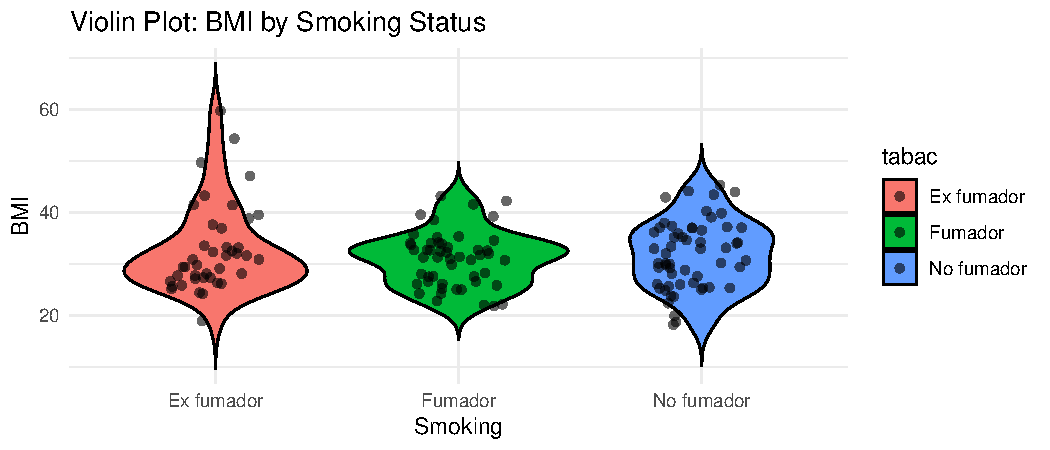
\includegraphics{StatisticsWithR-3-Exploratory_Analysis_II_And_Graphics_files/figure-beamer/unnamed-chunk-30-1.pdf}
\end{frame}

\begin{frame}[fragile]{Density Plot by CHD Status}
\phantomsection\label{density-plot-by-chd-status}
\begin{Shaded}
\begin{Highlighting}[]
\FunctionTok{ggplot}\NormalTok{(diab, }\FunctionTok{aes}\NormalTok{(}\AttributeTok{x =}\NormalTok{ bmi, }\AttributeTok{fill =}\NormalTok{ chd)) }\SpecialCharTok{+}
  \FunctionTok{geom\_density}\NormalTok{(}\AttributeTok{alpha =} \FloatTok{0.5}\NormalTok{) }\SpecialCharTok{+}
  \FunctionTok{labs}\NormalTok{(}\AttributeTok{title =} \StringTok{"BMI Distribution by CHD"}\NormalTok{, }\AttributeTok{x =} \StringTok{"BMI"}\NormalTok{, }\AttributeTok{y =} \StringTok{"Density"}\NormalTok{) }\SpecialCharTok{+}
  \FunctionTok{theme\_classic}\NormalTok{()}
\end{Highlighting}
\end{Shaded}

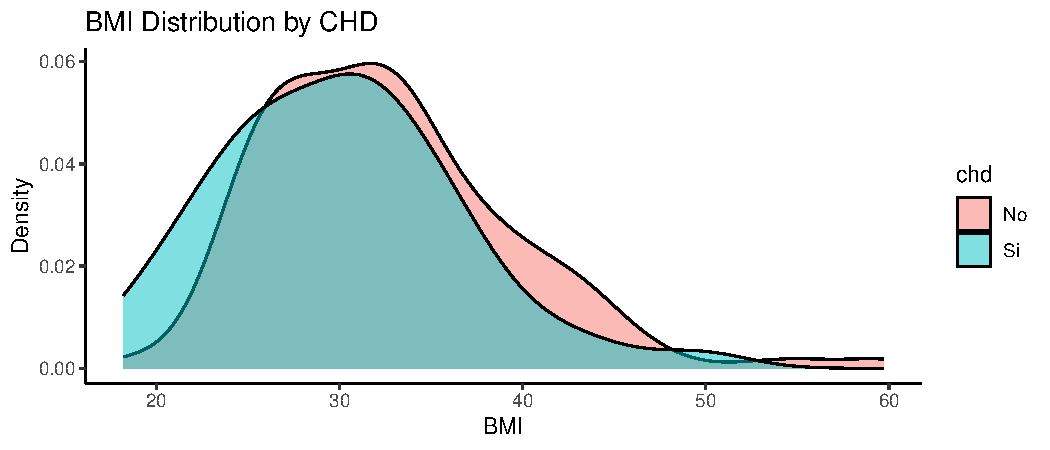
\includegraphics{StatisticsWithR-3-Exploratory_Analysis_II_And_Graphics_files/figure-beamer/unnamed-chunk-31-1.pdf}
\end{frame}

\begin{frame}[fragile]{Boxplot + Points + Mean Line}
\phantomsection\label{boxplot-points-mean-line}
\begin{Shaded}
\begin{Highlighting}[]
\FunctionTok{ggplot}\NormalTok{(diab, }\FunctionTok{aes}\NormalTok{(}\AttributeTok{x =}\NormalTok{ tabac, }\AttributeTok{y =}\NormalTok{ bmi, }\AttributeTok{fill =}\NormalTok{ tabac)) }\SpecialCharTok{+}
  \FunctionTok{geom\_boxplot}\NormalTok{(}\AttributeTok{outlier.shape =} \ConstantTok{NA}\NormalTok{) }\SpecialCharTok{+}
  \FunctionTok{geom\_jitter}\NormalTok{(}\AttributeTok{width =} \FloatTok{0.15}\NormalTok{, }\AttributeTok{color =} \StringTok{"black"}\NormalTok{, }\AttributeTok{size =} \DecValTok{2}\NormalTok{, }\AttributeTok{alpha =} \FloatTok{0.7}\NormalTok{) }\SpecialCharTok{+}
  \FunctionTok{stat\_summary}\NormalTok{(}\AttributeTok{fun =}\NormalTok{ mean, }\AttributeTok{geom =} \StringTok{"point"}\NormalTok{, }\AttributeTok{shape =} \DecValTok{20}\NormalTok{, }\AttributeTok{size =} \DecValTok{5}\NormalTok{, }\AttributeTok{color =} \StringTok{"red"}\NormalTok{) }\SpecialCharTok{+}
  \FunctionTok{labs}\NormalTok{(}\AttributeTok{title =} \StringTok{"BMI by Smoking Status with Mean"}\NormalTok{, }\AttributeTok{x =} \StringTok{"Smoking"}\NormalTok{, }\AttributeTok{y =} \StringTok{"BMI"}\NormalTok{) }\SpecialCharTok{+}
  \FunctionTok{theme\_light}\NormalTok{()}
\end{Highlighting}
\end{Shaded}

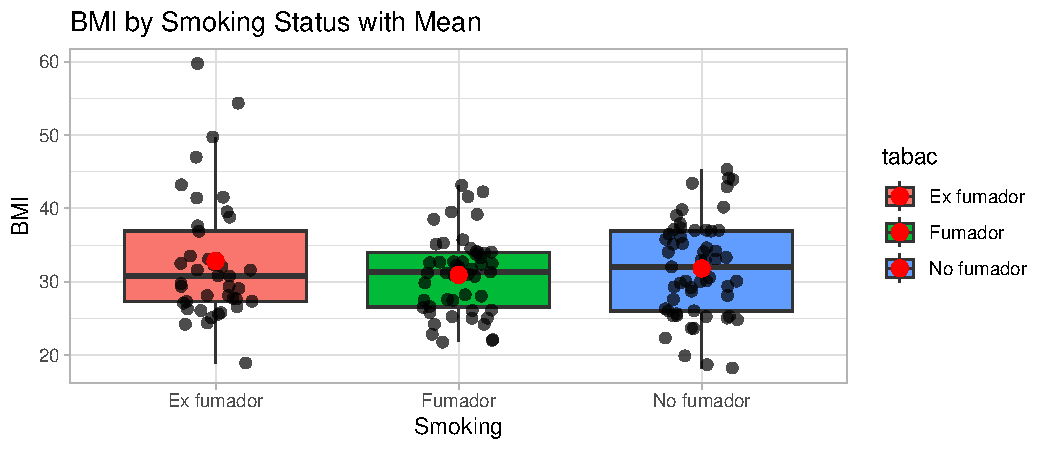
\includegraphics{StatisticsWithR-3-Exploratory_Analysis_II_And_Graphics_files/figure-beamer/unnamed-chunk-32-1.pdf}
\end{frame}

\section{Geospatial Visualization}\label{geospatial-visualization}

\begin{frame}[fragile]{World Map with Countries Colored}
\phantomsection\label{world-map-with-countries-colored}
\begin{Shaded}
\begin{Highlighting}[]
\FunctionTok{p\_load}\NormalTok{(maps)}

\CommentTok{\# Load world map data}
\NormalTok{world }\OtherTok{\textless{}{-}} \FunctionTok{map\_data}\NormalTok{(}\StringTok{"world"}\NormalTok{)}

\CommentTok{\# Plot a basic world map}
\FunctionTok{ggplot}\NormalTok{(world, }\FunctionTok{aes}\NormalTok{(}\AttributeTok{x =}\NormalTok{ long, }\AttributeTok{y =}\NormalTok{ lat, }\AttributeTok{group =}\NormalTok{ group)) }\SpecialCharTok{+}
  \FunctionTok{geom\_polygon}\NormalTok{(}\AttributeTok{fill =} \StringTok{"lightblue"}\NormalTok{, }\AttributeTok{color =} \StringTok{"white"}\NormalTok{) }\SpecialCharTok{+}
  \FunctionTok{labs}\NormalTok{(}\AttributeTok{title =} \StringTok{"Basic World Map"}\NormalTok{) }\SpecialCharTok{+}
  \FunctionTok{theme\_minimal}\NormalTok{()}
\end{Highlighting}
\end{Shaded}

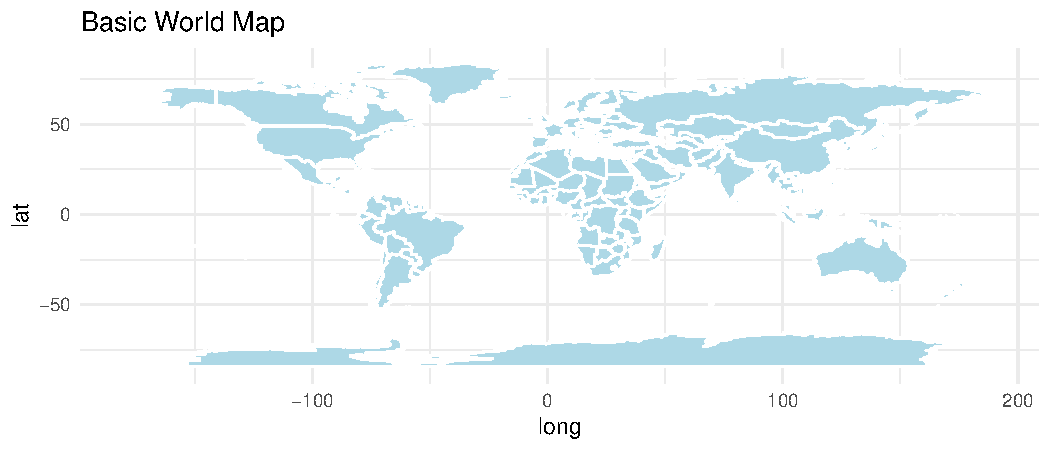
\includegraphics{StatisticsWithR-3-Exploratory_Analysis_II_And_Graphics_files/figure-beamer/unnamed-chunk-33-1.pdf}
\end{frame}

\section{Summary}\label{summary-1}

\begin{frame}[fragile]{Summary}
\begin{itemize}
\tightlist
\item
  Use \texttt{plotly} for interactive visualizations
\item
  \texttt{GGally::ggpairs} offers compact overviews
\item
  Combine multiple \texttt{ggplot2} layers for clarity and emphasis
\end{itemize}
\end{frame}

\end{document}
